\chapter{Zielsetzung}

Bei dem Projekt "`Sportangebot der HTW"' ging es darum, einen Beratungsassistenten zu erstellen. Hierbei handelt es sich um ein Softwareprodukt, das auf Fragestellungen Sportinteressierten nach Beantwortung eine geeignete Sportart vorschlägt.

\section{Szenarien}

Als Testfall wurden zwei Szenarien aufgestellt. Bei den Szenarien wurden bereits Überlegungen getroffen, ob die Fragen durch die Ontologie oder durch die Datenbank gefiltert werden nach der Natur der Sache. Bei der Umsetzung wurden allerdings teilweise veränderungen vorgenommen. Dazu später mehr.

Die Folgenden Tabellen stellen die Szenarien dar, wie sie das Team zum Zeitpunkt des ersten Meilensteins ausgearbeitet hat.

\begin{capfigure}[Szenario 1]
	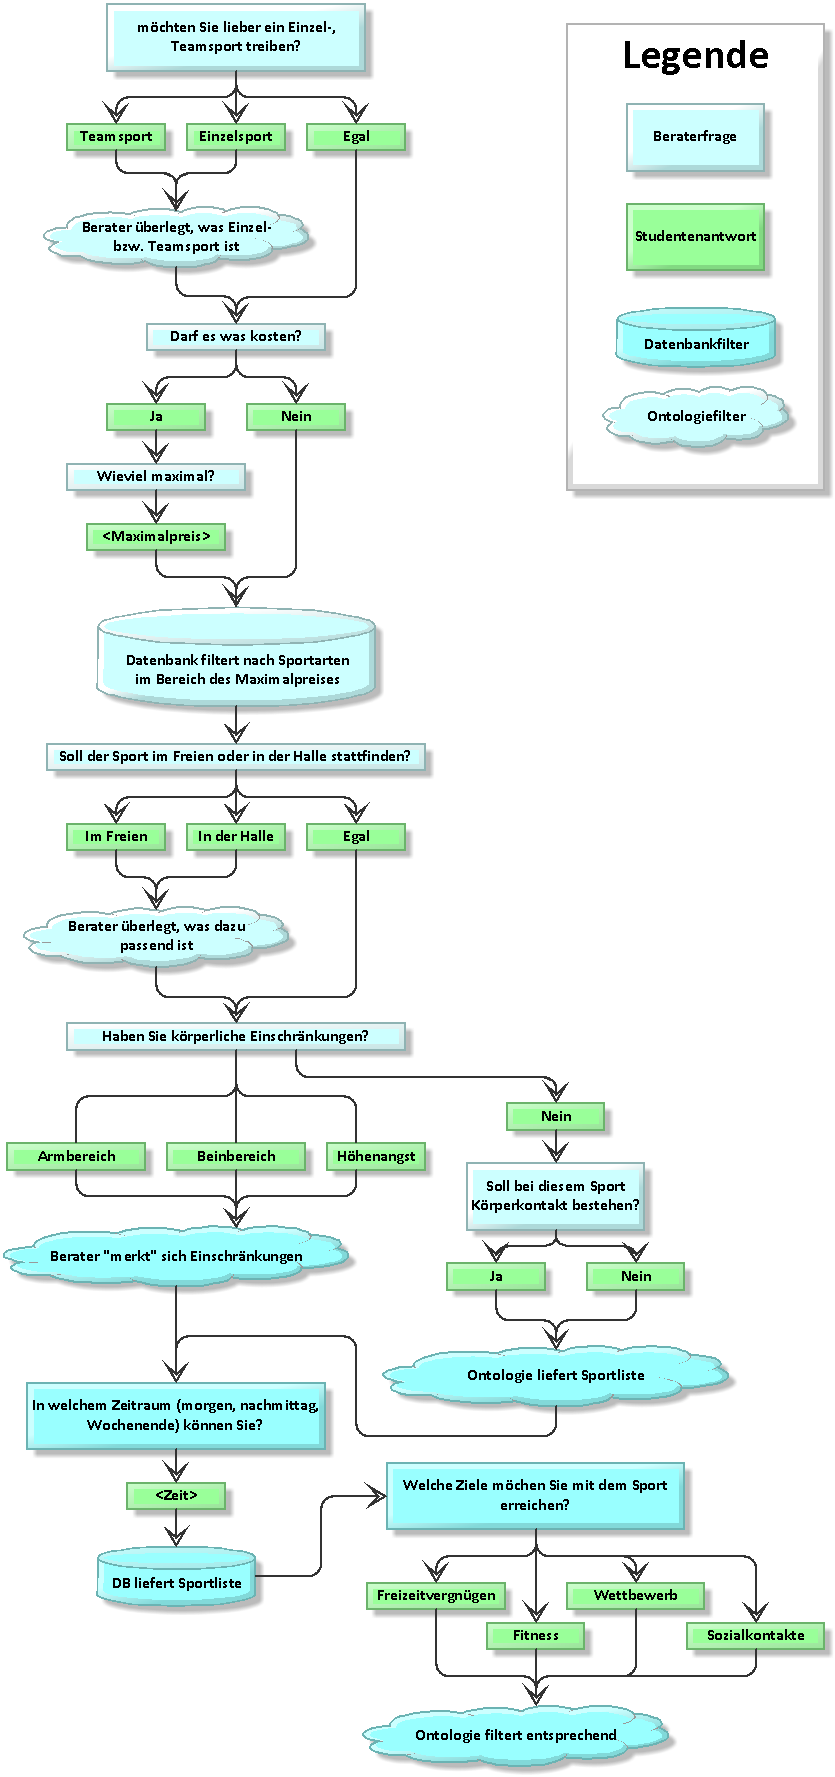
\includegraphics[width=100mm]{images/szenario1.png}
\end{capfigure}


\TODO{[PRIO:NORMAL]Tabellen sind so nicht sonderlich intuitiv und definitiv nicht schön. Hier wäre eine andere Variante der Darstellung besser. Idealerweise eine, die die Wege anzeigt.}

\

\begin{table}
	\centering
		\begin{tabular}{|r|l|l|}
\hline
			
1 &	Berater &	möchten Sie lieber ein Einzel-, Teamsport, usw. treiben? \\
&	Student	& Teamsport, Einzelsport ->2 Egal ->5 \\
\hline
2	& Berater	& Berater überlegt, was Team- oder Einzelsport ist -> Ontologie \\
\hline
5 &	Berater &	darf es was kosten? \\
\hline
6 &	Student	& nein, dann weiter zu Schritt 7 (mit max-Preis=0) \\
	& Student	& Ja \\
	& Berater	& Wieviel maximal?\\
	& Student &	nennt Maximalpreis\\
\hline
7	& DB &	 liefert eine Sport-Liste im Budget\\
	& Berater &	Mehr im Freien oder in der Halle?\\
	& Student &	mögliche Antworten: ja (->egal), im Freien, in der Halle\\
	& Onto & Berater überlegt, was dazu passend ist\\
\hline
8	& Berater &	Haben Sie körperliche Einschränkungen?\\
	& Student &	mögliche Antworten: Nein, Ja im Beinbereich,\\
	& & Ja im Armbereich, Ja psychische (z. B. Höhenangst)) \\ 
	&&(Doppenennnungen möglich, wenn sinnvoll)\\
\hline
-	& Onto & Nein -> 10, Ja -> 13, Berater "merkt sich" Einschränkungen \\
\hline
10 & Berater & Soll es bei diesem Sport Köperkontakt bestehen?\\
\hline
11 & Student & Ja bzw. Nein\\
\hline
12 & Ontologie & liefert eine Sport-Liste\\
\hline
13 & Berater & In welchem Zeitraum (morgen, nachmittag, Wochenende)\\
&& soll das Sportangebot stattfinden?\\
\hline
14 & Student & abends zwischen 17:00 und 21:00 \\
\hline
-	& DB &liefert eine Sport-Liste\\
\hline
15 & Berater & Welche Ziele möchen Sie mit dem Sport erreichen?\\
\hline
16 & Student & mögliche Antworten: Freizeitvergnügen, Wettbewerb,\\
&& Sozialkontakte, Fithalten\\
\hline
17 & Onto &	filtert entsprechend \\
\hline
-	& Berater &	schlägt dem Student die Sports vor, die ihm passen.\\
\hline
		\end{tabular}
		
		\caption[Szenario 1]{Szenario 1}
\end{table}


\begin{table}
	\centering
		\begin{tabular}{|r|l|l|}
\hline
1 &	Berater	& Wollen sie ein Einzel- oder Teamsport machen,\\
&& oder ein Tanz oder Entspannungsangebot wahrnehmen?\\
	& Student	& Einzel\\
\hline
	& Onto &	Gibt gefilterte Liste zurück\\
2	& Berater	& Dürfen die Angebote etwas kosten?\\
\hline
	& Student	& Nein\\ 
\hline
	& DB & Entsprechendes Filtern der vorherigen Liste.\\
\hline
3	& Berater	& Darf es sich um eine Kampfsportart handeln?\\
\hline
	& Student	& Nein\\
\hline
	& Onto & Entsprechendes Filtern der vorherigen Liste.\\
\hline
4	& Berater	& Haben Sie Höhenangst?\\
\hline
	& Student	& Ja\\
\hline
	& Onto	&Ja: Entsprechendes Filtern der vorherigen Liste.\\
\hline
	& & Nein: Liste übernehmen\\
\hline
5	& Berater& Soll das Angebot innen oder aussen stattfinden.\\
\hline
	& Student& Innen\\
\hline
	& DB & Innen, Aussen: entsprechend filtern.\\
\hline
	& &Egal: übernehmen\\
\hline
6	&Berater&	Soll das Angebot ein Wettbewerb sein.\\
\hline
	&Student&	Ja\\
\hline
	&Onto	&filtert entsprechend\\
\hline
7	&Berater&Vertragen Sie es beim Angebot nass zu werden?\\
\hline
	&Student&Nein\\
\hline
	&Onto	&Badminton, Fechten, Headis, Renaissance-Fechten...\\
\hline
8	&Berater &Soll das Angebot exotischer sein?\\
\hline
	&Student&Ja\\
\hline
	&Onto&filtert entsprechend\\
\hline
9	&Berater&Wann haben Sie Zeit?\\
\hline
	&Student&	Dann und dann.\\
\hline
	&DB&Keine Ausgabe\\
\hline
10&Berater&Keine passendes Angebot gefunden\\
\hline
	&Student&Zurück zu Schritt x.\\
\hline
	\end{tabular}
	
\caption[Szenario 2]{Szenario 2}

\end{table}